This chapter deals with the collaboration and process in the project. First we introduce some theory on project management and global collaboration. In the next step we report our project work: We introduce the project team, the initial situation and present the chosen project management approach, methods and tools. In addition we evaluate the collaboration tools we used in the project. Finally, we lead to the issues we had to face during the project. These include progress issues, issues with the used project management techniques and collaboration issues. We analyze the collaboration issues based on the previous introduced theory. Furthermore we reflect the process and collaboration and explain our learning outcomes.

%---

\section{Theory}

\subsection{Project management}

There are two major approaches how you can perform project management: The traditional approach and the agile approach.

The traditional approach is ... \todo{TODO}

An agile project management approach is ... \todo{TODO}

A popular agile project management framework is Scrum. \todo{TODO}

\subsection{Global collaboration} \todo{TODO}

	\begin{itemize}
		\item Trust
		\item Individualism
		\item Power distance
	\end{itemize}

%---

\section{Background information of the Project Team}
The project team consists of two groups of students. One group is from the Strathmore University located in Nairobi (Kenya). The other group is from the IT University (ITU) in Copenhagen (Denmark). The project team agreed on to name the two groups "Team Kenya" for the student group from Strathmore University and "Team ITU" for the student group from ITU. This helped to address each group in meeting reports, emails and conversations.

In the following paragraphs the background information for this project from both groups are introduced. The information explains the motivation and contribution of each group in the project and is used as argumentation why certain decisions were made and issues aroused.


\subsection{Team ITU}
Team ITU started with four members, which are all in the Masters programme "Software Development and Technology (Software Engineering)" of the ITU.\footnote{In the beginning there were five members, but one left the project after two weeks, because he changed to another project and project team. This did not have an impact on the work as it was in the early stage of the project.} The members are from three different countries: Lithuania, Germany and Denmark.\footnote{Although there are minor differences between the nationalities, which could have an influence on the team work, we will not go into this, because it is out of scope for this report.} The communication language within Team ITU is English, which is not the mother tongue of any of the members. The members of Team ITU met each other the first time on the 27.8.2013.

The students of Team ITU have to complete the project under the course "Global Software Development Project", which is mandatory for their masters programme. The requirements and deadlines for the project are given in the course base from ITU (reference\todo{Link to the course base}) and by the advisor of the project. The course is rated with 15 ECTS points, which corresponds to approximately 20 hours per week per student. The students of Team ITU have to hand in this report as a mandatory requirement.

As the course for the Team ITU started in late August and the project team and topic was already known, Team ITU already started with the project work before Team Kenya. Team ITU and their advisor did not know when to get the contact details from the student group in Kenya, so the advisor recommended already initializing the project and doing some research and thoughts on the project.

At the beginning Team ITU had received a different project topic by the advisor. The topic of the first project was "Vector Shooter".\footnote{In this project a program had to be developed, in which the calculation of a vector - based on an image - has to be made. The image should contain a person, who uses his hands to demonstrate a vector by taking a position like he uses a bow and arrow. The requirement was to use webcams, to capture the image, and to use RaspberryPis to detect the hands of the person and to calculate the vector. Furthermore, an Android application should be included in the program.} Team ITU put some thoughts into the project and spent time on defining the program, which they wanted to develop.

After three weeks the advisor had to change the topic of the project due to the collaboration with the Strathmore University. Only one student from the Strathmore University was interested on the project "Vector Shooter". Team ITU could have spent time and effort in convincing the other students from Strathmore University to do the project "Vector Shooter". Despite frustration, in consideration of the given deadline of the course and on recommendation of the advisor, Team ITU decided to not take this option.

Team ITU received the project topic and the contact details of the members of Team Kenya on the 17.9.2013. So the collaboration between the student groups did not start before this date.


\subsection{Team Kenya}

In the beginning Team Kenya consists of three members, which are all in the Masters programme "Telecommunication and Innovation" of the Strathmore University. The members are all from Kenya. The official languages in Kenya are English and Swahili. The members of Team Kenya met each other the first time on the 1.10.2013 (--> Appendix \ref{app:appendixB}: \hyperlink{GSD20131001.1}{Global Meeting Report 1.10.2013 Page 1}). One member had to leave the group in the last third of the project due to workload of other projects and obligations (--> Appendix \ref{app:appendixB}: \hyperlink{GSD20131126.2}{Global Meeting Report 26.11.2013 Page 2}).

The department, which is responsible for the masters programme "Telecommunication and Innovation", wants to convince the school management from Strathmore University to invest into the technology and idea of the project to improve environmental conservation. Therefore this collaboration project was initiated. (--> Appendix \ref{app:appendixB}: \hyperlink{GSD20131203.2}{Global Meeting Report 3.12.2013 Page 2}) \todo{Maybe in the Introduction-Context Part?}.

For the students from Team Kenya the project is not included in a mandatory course and is completely voluntarily. The students from Team Kenya spend their free time on this project. There are no mandatory requirements or deadlines, which the Kenyan students have to achieve, except that they have to create documentation for their advisor to prove the progress of the project (--> Appendix \ref{app:appendixB}: \hyperlink{GSD20131119.2}{Global Meeting Report 19.11.2013 Page 2}). The motivation for the Kenyan students to participate in this project is on the one hand to support the environmental thought and on the other hand to use this project work as basis for their master thesis (Email 10.12.2013 \todo{Add refernce}).

%---

\section{Project Management}

\subsection{Approach}

As the course for the team ITU started in late August and the project team was already known, Team ITU already started with a project management technique, which was already established when Team Kenya got into the project.

Team ITU chose an agile project management approach, because it is more flexible, which was important due to the fact, that Team ITU did not knew the student group from Strathmore University neither their skills nor their requirements on this project. Moreover an agile project management approach is known for being more suitable for software development projects (*TODO: reference*\todo{Find reference}).

Team ITU planned to merge Team Kenya into their project management approach as they did not come up with a different approach. Team ITU considered introducing Scrum to the project. However, due to the inexperience and non-knowledge about this framework in both teams, this idea has been dropped. For Scrum it is necessary that every project team member knows the concept. Thus, each team member would need to learn Scrum, which in turn would have meant losses for the implementation.

%---

\subsection{Project Organization}

\subsubsection{Timeline}
Team Kenya agreed on to go with the deadlines from Team ITU as they do not have to meet any deadlines. (--> Appendix \ref{app:appendixB}: \hyperlink{GSD20131024.1}{Global Meeting Report 24.10.2013 Page 1})

\subsubsection{Project Team and Roles}
Each member of the project team created a member profile to introduce themselves, which are attached in the Appendix \ref{sec:member_profiles}.

The members of Team ITU split up the tasks, such that different kind of roles aroused. The roles were not set in the beginning, but emerged during the project progress. They explain the major responsibilities. This does not

\textbf{Collaboration master}

\textbf{Server Developer}

\textbf{Image Processing Developer}

\textbf{Prediction Model Developer}

\textbf{Team Kenya/Android Application Developers}


%---

\subsection{Project Management Tools and Methods}

\subsubsection {Member profiles}
Team ITU suggested to come up with some member profiles of each project team member to introduce themselves in the beginning of the project. One member of Team Kenya followed the suggestion in the beginning. The other two members provided their member profile three weeks after Team ITU requested them. It could be noted that this already led to disappointment on the side of Team ITU.

\subsubsection {Skill-/Preference- and Motivation-Sheet}
To see where the strengths, weaknesses and motivations within the project team are Team ITU came up with a Skill-/Preference-Sheet and Motivation-Sheet. Every project team member was encouraged to fill out these tables. The results can be seen in the Appendix \ref{sec:Skill_Preference_Sheet} and \ref{sec:Motivation_Sheet}.

The outcome of these tables also influenced some decisions in the project. For example on which programming languages Team ITU made a benchmark on (*reference*)\todo{Add refernce}, which database technology and which version control system for the source code is used. It also pointed out the possible roles of each project team member within the project (*reference*)\todo{Add refernce}.

In the result it can be noticed that image processing, prediction models and RaspberryPis were quite unknown amongst the project team members. So each project team member was encouraged to do some research on these topics in the beginning.

\subsubsection{"Out-of-Office"-Calendar}

Because every project team member had different obligations besides the project, Team ITU came up with an "Out of Office"-Calendar, in which every project team member could publish for example exams, other hand-ins or other unavailability. The motivation of this calendar was to do a better planning on meetings and assignments during the project. The problem was that no one really looked into this calendar except in the beginning of the project or when a certain issue aroused. The "Out-of-Office"-Calendar can be seen in the Appendix \ref{sec:Calendar}.

So it was noticed that Team Kenya as well as Team ITU had some exams in October. This influenced the project plan according to when to start the implementation phase. Later in the project it was forgotten or not correctly interpreted by Team ITU, that Team Kenya had a second exam phase in the first half of November. Team ITU got informed by this, when Team Kenya did not come up with agreed assignments (--> Appendix \ref{app:appendixB}: \hyperlink{GSD20131112.2}{Global Meeting Report 12.11.2013 Page 2}).


\subsubsection{Milestone plan}
Team ITU chooses to create a very rough milestone plan to have an eye on the deadline given by ITU. A detailed milestone plan would contradict the idea of the agile project management approach. Team ITU did not know Team Kenya, their skills and requirements in the beginning and a detailed milestone plan probably would have been run over several times. In the milestone plan Team ITU roughly pointed out when they want to be done with each phase of the project.

The following milestones, where set in the beginning of the project.

	\begin{figure}[ht]
		\centering
		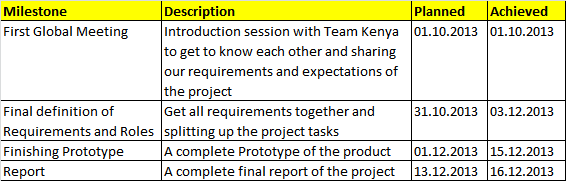
\includegraphics[scale=1]{collaboration/Milestones_table}
		\caption{Milestone Plan}
		\label{fig:milestones_table}
	\end{figure}

Figure~\ref{fig:milestones} shows the milestone plan, which was planned in the beginning of the project.

	\begin{figure}[ht]
		\centering
		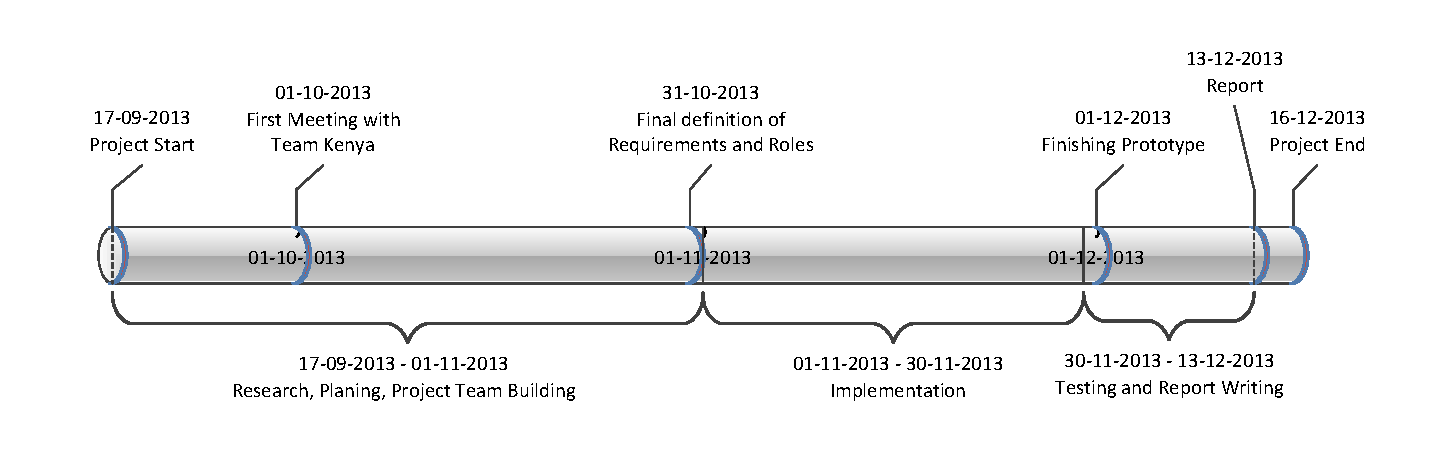
\includegraphics[scale=0.7]{collaboration/Milestones}
		\caption{Milestone Timeline}
		\label{fig:milestones}
	\end{figure}

The milestone plan was mostly a guideline for Team ITU, because they had a deadline in contrast to Team Kenya. Team ITU shared the planed dates for half of the milestones with Team Kenya as they agreed to go with the deadlines from Team ITU. (--> Appendix \ref{app:appendixB}: \hyperlink{GSD20131024.1}{Global Meeting Report 24.10.2013 Page 1}) These shared milestones were according to when to finish the prototype and when to hand-in the mandatory final report.

\subsubsection{Internal weekly meeting (Jour-Fixe)}
Team ITU agreed on having an internal weekly meeting to update each other on the current progress, to discuss occuring topics, make decissions, work together and assign each other new assignments till the next meeting. Furthermore Team ITU also met with their advisor to check if they are on the right track. The concept of the weekly meeting equates to the concept of a Jour Fixe \todo{Find reference} or a Daily Scrum \todo{Find reference}.

There was a constant agenda for the meeting:

	\begin{enumerate}
		\item Status update of each team member
			\begin{enumerate}
				\item What has each group done during the past week according to the project?
				\item Which achievements were made?	
				\item Which problems occurred?
				\item Any other news
			\end{enumerate}
		\item Discussions and Decisions (the topics in this section varied weekly according to the current progress)
		\item Meeting with advisor	
		\item Assignments
	\end{enumerate}

This constant agenda gave some structure to the project. The team members know what to expect from the meeting and where they can place their concerns.

The members of Team ITU were mostly fully represented in the internal weekly meeting. 

\subsubsection {Global weekly meeting (Jour-Fixe)}
Team Kenya and Team ITU agreed on having a weekly Skype-Meeting (*reference*\todo{Add reference}) to update each other on the current progress, to discuss occurring topics, make decisions and assign each other new assignments till the next meeting, just like the weekly internal meeting. The meeting took place every Tuesday afternoon/evening. According to a Doodle-Survey (*reference*\todo{Add reference}) all project team members could reserve this time for the project meeting.

Each group could make a suggestion for the Agenda, but Team Kenya never used this opportunity. Therefore only Team ITU prepared an agenda, which was structured in the following way:

	\begin{enumerate}
		\item Status update of each group
			\begin{enumerate}
				\item What has each group done during the past week according to the project?
				\item Which achievements were made?	
				\item Which problems occurred?
				\item Any other news
			\end{enumerate}
		\item Discussions and Decisions (the topics in this section varied weekly according to the current progress)
		\item Assignments
	\end{enumerate}

After the first few meetings Team Kenya and Team ITU agreed on to prepare the status update in advance, because it took quite a while for each group to present their status updates in the Skype chat. Unfortunately Team Kenya did not comply with this agreement except in the last meeting, where none of the Kenyans could attend due to other obligations or internet connection problems (Figure~\ref{fig:global_meetings}).

	\begin{figure}[ht]
		\centering
		\includegraphics[scale=1]{collaboration/Global_meetings}
		\caption{Milestone Plan}
		\label{fig:global_meetings}
	\end{figure}

As it can been seen in Figure~\ref{fig:global_meetings} almost every meeting took place. Team ITU was always in the majority. The attendance from Team Kenya was low mostly due to other obligations and internet connection problems.

\subsubsection {Meeting reports}

For every internal and global weekly meeting Team ITU wrote a meeting report. These meeting report documents all updates, news, discussions, decisions and assignments, which were discussed in the meetings. After publishing the meeting report, each project team member had the chance to correct wrong information or add missing information for the next couple of days. Afterwards the information and assignments in the meeting report were binding.

Project team members which could not attend the meeting had the chance to be updated with all necessary information. The report also confirms the content of the meeting. Furthermore the report is a source the team members can rely on. For example in case it comes to false allegations against a team member, the report could be used as a proof. The meeting report is also a reminder on the agreed tasks.

Team ITU expected that the agreed assignments were done or at least started to the next meeting. Since this did not happen on the side of Team Kenya, Team ITU started to put some deadlines on the most important assignments. But even those assignments were not done in time or done at all, although Team ITU got specific confirmation by email on the published meeting report or no disagreement on the meeting report from Team Kenya.

\subsubsection {Time recording}
\subsubsection {Introduction and Kick-Off meeting}
\subsubsection {Surveys}

%---

\subsection{Collaboration Tools}

\subsubsection {Communication}
	\begin{itemize}
		\item Skype (excluding Google Hangout)
		\item Email
	\end{itemize}
\subsubsection {Sharing}
	\begin{itemize}
		\item Google Drive (excluding Skydrive)
		\item Github
	\end{itemize}
\subsubsection {Time recording}
	\begin{itemize}
		\item Toggl (excluding Excel)
	\end{itemize}

%---


\section{Project Issues}

\subsection{Collaboration Issues}
%The issues and how you responded to them

	\begin{itemize}

		\item Illusion of the project work and project team
		\item Failure to comply with the assignments
		\item Communication
		\item Lack of skills
		\item Other exams/hand-ins
		\item Differing requirements
		\item Attendence of meetings
		\item Equipment

	\end{itemize}

%---

\section{Hypothetical Scenarios}
%Relevant hypothetical scenarios

	\begin{itemize}
		\item Assignments
		\item Communication
		\item Requirements
		\item Organisation by the universities (Requirments, clarification, )
	\end{itemize}
